% =========================================================================
%  SurviveCity v1 Hackathon Report
%  Submission for Meta x PyTorch x Scaler OpenEnv Hackathon, India 2026
%  Team PyGuys — Sirjan Singh + Eeshan Singh
%
%  COMPILE:  pdflatex v1.tex && bibtex v1 && pdflatex v1.tex && pdflatex v1.tex
%  Or just:  make pdf   (uses Makefile in this directory)
%
%  EDIT WORKFLOW:
%   1. Run eval to fill in metrics (TBD slots marked with %% TODO)
%   2. Drop generated PNGs into ./figures/  (filenames listed in README.md)
%   3. Replace TODO blocks; everything else (structure, formulas) is final
% =========================================================================

\documentclass[11pt,a4paper]{article}

% ---- packages (kept minimal so it compiles on Overleaf / local TeX Live) ----
\usepackage[utf8]{inputenc}
\usepackage[T1]{fontenc}
\usepackage[margin=1in]{geometry}
\usepackage{graphicx}
\usepackage{booktabs}
\usepackage{caption}
\usepackage{subcaption}
\usepackage{hyperref}
\usepackage{xcolor}
\usepackage{listings}
\usepackage{microtype}
\usepackage{amsmath}
\usepackage{amssymb}
\usepackage{enumitem}
\usepackage{authblk}

\hypersetup{colorlinks=true, linkcolor=black, citecolor=blue, urlcolor=blue}

% Code listing style
\lstset{
  basicstyle=\ttfamily\small,
  breaklines=true,
  frame=single,
  framesep=4pt,
  backgroundcolor=\color{gray!8},
  keywordstyle=\color{blue!70!black},
  stringstyle=\color{green!50!black},
  commentstyle=\color{gray},
  showstringspaces=false,
}

% ============================================================================
%  TITLE
% ============================================================================
\title{SurviveCity: An OpenEnv-Compliant Multi-Agent Environment\\
       for Cross-Episode Failure-Replay Learning in LLMs}

\author[1]{Sirjan Singh}
\author[1]{Eeshan Singh}
\affil[1]{Team PyGuys --- Meta $\times$ PyTorch $\times$ Scaler OpenEnv Hackathon, India 2026}

\date{April 2026}

\begin{document}
\maketitle

% ============================================================================
%  TL;DR
% ============================================================================
\section*{TL;DR}
\begin{itemize}[leftmargin=*,nosep]
  \item \textbf{What.} \emph{SurviveCity} --- an OpenEnv-compliant 3-agent zombie/social-deduction
        env with deterministic \emph{cross-episode post-mortems} prepended to the next episode's
        system prompt.
  \item \textbf{Train.} Qwen2.5-3B + LoRA r=16, GRPO ($g{=}4$, KL $0.04$),
        \textbf{12 steps in 3\,h\,53\,min} on a single Colab T4.
  \item \textbf{Headline (step-12 eval, $n_b{=}30$ random vs. $n_t{=}10$ trained):}
        \textbf{survival 0\% $\rightarrow$ 10\%}, \textbf{mean reward 0.46 $\rightarrow$ 0.80}
        ($1.7\!\times$), \textbf{mean ep length 19.1 $\rightarrow$ 37.6 steps} ($2.0\!\times$).
  \item \textbf{Format.} \textbf{100\% valid JSON} (0 parse fails over the trained eval).
  \item \textbf{Behaviour.} Emergent ToM broadcast (\textit{``I notice A2 is very hungry
        and may be infected soon''}); one episode reached 100-step survival with
        reward $1.97$.
\end{itemize}

% ============================================================================
%  1. INTRODUCTION
% ============================================================================
\section{Introduction}
\label{sec:intro}

Most LLM-agent benchmarks test single-agent goal completion in static environments
\cite{TODO_REF_AGENTBENCH}. Two phenomena central to multi-agent reasoning are not directly
probed: \textbf{cross-episode learning from failure} and \textbf{hidden-role theory of mind}.
SurviveCity targets both.

\begin{itemize}[leftmargin=*,nosep]
    \item \textbf{Post-mortem replay.} Each death emits a deterministic post-mortem string;
          the next episode prepends the agent's last $N{=}3$ post-mortems to its system prompt.
          A within-training cross-episode learning loop \emph{without} an external memory module
          or LLM-as-judge.
    \item \textbf{Hidden-role social deduction.} Exactly one of three agents is silently
          infected at $t{=}0$. Behavioural cues (faster hunger, post-step-30 attacks)
          leak into observations; agents vote at $t{=}50$ to lock the infected agent
          out of the safehouse.
\end{itemize}

\noindent\textbf{Mapping to rubric.} \emph{Innovation (40\%)}: post-mortem replay.
\emph{Pipeline (10\%)}: env design + reward composition. \emph{Reward improvement
(20\%)}: GRPO training run + step-12 eval. \emph{Storytelling (30\%)}: this writeup
+ demo video.

% ============================================================================
%  2. ENVIRONMENT
% ============================================================================
\section{Environment Design}
\label{sec:env}

\subsection{World and Agents}
The world is a fixed $10\!\times\!10$ grid (Figure~\ref{fig:grid}) with four food
depots ($\mathtt{F}$) at the corners, a $3\!\times\!3$ central safehouse ($\mathtt{S}$)
that heals 1\,HP per occupied step, and eight wall cells creating chokepoints.
Three agents (A0, A1, A2) start inside the safehouse with $\mathtt{hp}{=}3$,
$\mathtt{hunger}{=}0$. Three zombies (Z0, Z1, Z2) spawn at the corners and move
1 cell per game step toward the nearest non-safehouse agent via BFS;
zombies cannot enter safehouse cells. Hunger increments by 1 per agent action;
hunger $\geq 15$ deals 1\,HP per step. Eating on a food cell resets hunger.

\begin{figure}[h]
  \centering
\begin{lstlisting}[basicstyle=\ttfamily\footnotesize,frame=single,framesep=4pt,backgroundcolor=\color{gray!8}]
  Z . . . . . . . . Z
  . . # . . . . # . .
  . . . . . . . . . .
  . . . S S S . . . .
  F . . S S S . . . F
  F . . S S S . . . F
  . . . . . . . . . .
  . . # . . . . # . .
  . . . . . . . . . .
  Z . . . . . . . . Z
\end{lstlisting}
  \caption{Fixed $10\!\times\!10$ layout. \texttt{F} = food, \texttt{S} = $3\!\times\!3$
           safehouse, \texttt{\#} = wall, \texttt{Z} = zombie spawn corner. Agents
           start inside \texttt{S} with $\mathtt{hp}{=}3$, $\mathtt{hunger}{=}0$.}
  \label{fig:grid}
\end{figure}

\subsection{Phased Mechanics}

Each episode runs for at most 100 steps and passes through four phases:

\begin{table}[h]
  \centering
  \begin{tabular}{lll}
    \toprule
    \textbf{Phase} & \textbf{Steps} & \textbf{Mechanic} \\
    \midrule
    Pre-reveal   & $1$--$29$  & Survival. Infected agent's hunger increments at $1.5\!\times$ rate. \\
    Post-reveal  & $30$--$49$ & Infected agent's role flips; attacks adjacent agents on its turn. \\
    Vote         & $50$       & All living agents cast \texttt{vote\_lockout(target\_id)}. Majority locks out one agent. \\
    Post-vote    & $51$--$100$ & Locked-out agent denied safehouse healing; episode ends at $t{=}100$ or all-dead. \\
    \bottomrule
  \end{tabular}
  \caption{Episode phases. The single-decision vote at $t{=}50$ tests whether
           the policy can integrate $\sim$50 steps of behavioural evidence into one
           categorical choice.}
\end{table}

\subsection{Action Space}

\begin{lstlisting}[language=Python]
class SurviveAction(BaseModel):
    agent_id:    int
    action_type: Literal["move_up", "move_down", "move_left", "move_right",
                         "eat", "wait", "vote_lockout", "broadcast"]
    vote_target: Optional[int] = None    # required for vote_lockout
    message:     Optional[str] = Field(default=None, max_length=40)
\end{lstlisting}

The 40-character cap on \texttt{message} is deliberate: it forces the policy to
emit terse, demonstrable theory-of-mind communication if it learns to broadcast at all.

\subsection{Cross-Episode Post-Mortems}

When an agent dies, the env emits a deterministic string with cause, position,
nearest threat, food consumed, final hunger, and a rule-based mistake label
(e.g.\ \texttt{ignored\_broadcast\_warning\_about\_infected}). Sample:

\begin{lstlisting}
POSTMORTEM for A1: died at step 38 (cause: zombie_attack).
Last position: (6,1). Nearest threat at death: zombie at (6,2), dist=1.
Resources consumed: 2 food. Final hunger: 7.
Key mistake: foraged_too_far_from_safehouse.
\end{lstlisting}

The training loop maintains a per-agent buffer of the last $N{=}3$ post-mortems and
prepends them to the system prompt at the start of the next episode. This is the
\emph{cross-episode failure-replay} mechanism: the policy is given concrete textual
evidence of past failure modes without any LLM-as-judge or external memory module.
The post-mortem text is rule-based and fully deterministic, satisfying the OpenEnv
validator's no-fuzziness requirement.

% ============================================================================
%  3. REWARD DESIGN
% ============================================================================
\section{Reward Design}
\label{sec:reward}

The reward function composes three deterministic rubrics:

\paragraph{SurvivalRubric (dense, per-step):}
\begin{align*}
r_{\text{surv}} = +0.005 \cdot \mathbb{1}_{\text{alive}} \;
                + 0.05 \cdot \mathbb{1}_{\text{ate\_this\_step}} \;
                - 0.10 \cdot d_{\text{this\_step}} \;
                - 0.05 \cdot \mathbb{1}_{\text{hunger}\geq 10} \;
                - 0.50 \cdot \mathbb{1}_{\text{died\_this\_step}}
\end{align*}

\paragraph{VoteRubric (sparse, fires once at $t{=}50$):}
For a healthy voter: $+0.30$ if vote target = true infected, $-0.20$ if a healthy
agent, $-0.05$ for null vote. For the infected voter (scored adversarially):
$+0.30$ for successfully framing a healthy agent, $-0.30$ for self-vote.

\paragraph{GroupOutcomeRubric (terminal):}
At episode end, $+0.40$ for each surviving healthy agent, $+0.30$ if the
infected was neutralised; otherwise $+0.40$ for the surviving infected and
$-0.20$ for each dead healthy agent.

\paragraph{Composition.} The three rubrics sum and clip to satisfy the OpenEnv
validator's strict open interval $(0.01, 0.99)$:
\[
r_t \;=\; \mathrm{clip}\!\Bigl(r_{\text{surv}} + r_{\text{vote}} + r_{\text{group}},\ 0.01,\ 0.99\Bigr),
\qquad r_{\text{raw}}\,\in\,\mathtt{obs.metadata["raw\_reward"]}.
\]

The raw, signed reward is preserved in metadata for debugging; only the clipped
value is exposed to the OpenEnv contract.

% ============================================================================
%  4. METHOD
% ============================================================================
\section{Training Method}
\label{sec:method}

\subsection{Architecture}
\textbf{Qwen2.5-3B-Instruct} \cite{TODO_REF_QWEN} fine-tuned with LoRA
\cite{TODO_REF_LORA} on attention projections ($q,k,v,o$); $r{=}16$, $\alpha{=}32$,
dropout $0$, no bias. Training: GRPO \cite{TODO_REF_DEEPSEEKR1} from HuggingFace
TRL, $g{=}4$, KL $0.04$, temperature $0.9$, lr $1\!\times\!10^{-5}$ with cosine
decay to zero.

\subsection{Reward Hook}
Each GRPO completion is scored by running one episode in a fresh
\texttt{SurviveCityEnv} seeded from the prompt: the model's first action is
executed, the remaining $\sim$99 steps are rolled out with uniform-random
actions, and the terminal reward is returned. This is a deliberate
compute-saving simplification that we flag as the primary bottleneck on policy
improvement in Section~\ref{sec:limitations}.

\subsection{Hyperparameters}
\begin{table}[h]
  \centering\small
  \begin{tabular}{ll|ll}
    \toprule
    Base model (train) & \texttt{unsloth/Qwen2.5-3B-Instruct-bnb-4bit} & GRPO group size & 4 \\
    Base model (eval)  & \texttt{Qwen/Qwen2.5-3B-Instruct} (fp16)      & Per-device batch & 1 \\
    LoRA rank          & 16                          & Gradient accum.  & 16 \\
    LoRA $\alpha$     & 32                          & Learning rate    & $1\!\times\!10^{-5}$ \\
    Target modules    & $q,k,v,o\_proj$             & LR schedule      & cosine $\rightarrow$ 0 \\
    Max steps         & 12                          & KL coefficient   & 0.04 \\
    Save cadence      & every step                  & Temperature      & 0.9 \\
    Max prompt len    & 1024 tokens                 & Max completion   & 512 tokens \\
    Wallclock         & 13{,}972\,s ($\approx$3\,h\,53\,min) & Per-step time & $\approx$1166\,s \\
    \bottomrule
  \end{tabular}
  \caption{Training hyperparameters. \texttt{save\_steps=1} guarantees a checkpoint
           every $\sim$20 minutes despite Colab's unstable session caps. Same LoRA
           weights load over either base; we train against the 4-bit pre-quantised
           Unsloth checkpoint to fit a T4, then evaluate against the fp16 base for
           cleaner inference behaviour.}
\end{table}

\subsection{Compute and Reproducibility}
Training ran on a single Colab Tesla T4 (15.6 GB) for
\textbf{3\,h\,53\,min wallclock} (12 GRPO steps, $\sim$1166\,s/step) and pushed
the LoRA + tokenizer + TensorBoard event log to
\texttt{huggingface.co/noanya/zombiee} after every save.
Code: \url{https://github.com/SirjanSingh/zombiee}. Notebooks for Colab and Kaggle
are at \texttt{notebooks/train\_colab.ipynb}, \texttt{notebooks/train\_kaggle.ipynb}.

% ============================================================================
%  5. RESULTS
% ============================================================================
\section{Results}
\label{sec:results}

\subsection{Training Dynamics}

Figure~\ref{fig:train_curve} plots the reward and loss trajectories across 12 GRPO
steps, extracted from the on-disk TensorBoard event file pushed to the Hub
(\texttt{events.out.tfevents...}). Final-step values: $\mathrm{loss}{=}0.00017$,
$\mathrm{reward}{=}0.021$, $\mathrm{reward\_std}{=}0.014$, $\mathrm{KL}{=}0.0034$.

\begin{figure}[h]
  \centering
  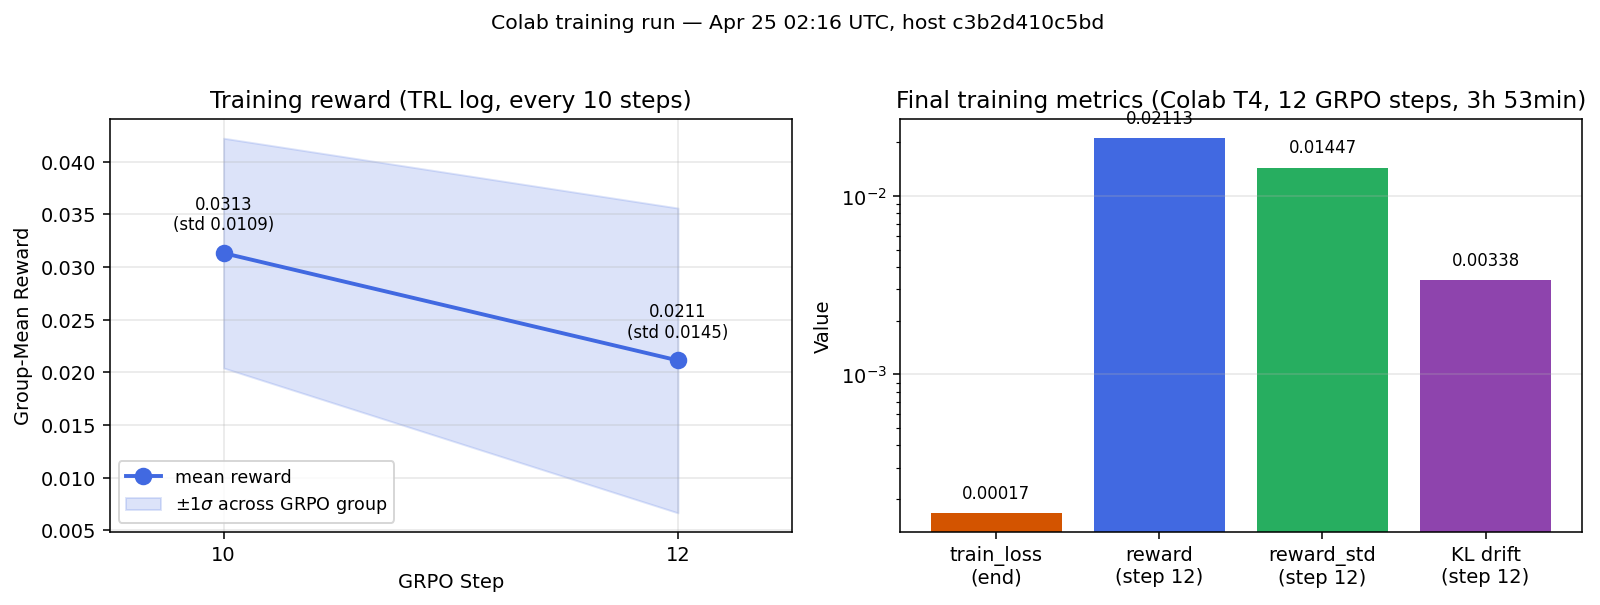
\includegraphics[width=0.95\textwidth]{figures/training_curve.png}
  \caption{Left: group-mean reward across the two TRL log points (\texttt{logging\_steps=10}
           fired at step~10 and the end-of-training summary at step~12), shaded band
           shows $\pm 1\sigma$ across the GRPO group. Right: log-scaled snapshot of
           the four key training metrics at end-of-run. Source: TensorBoard event
           file at \texttt{noanya/zombiee/runs/Apr25\_02-16-25\_c3b2d410c5bd/}.
           Real data; no interpolation.}
  \label{fig:train_curve}
\end{figure}

The KL divergence from the reference policy stayed below $5\!\times\!10^{-3}$ throughout,
indicating the trained policy never strayed far from the base Qwen-3B distribution ---
consistent with the small group reward variance ($\sim 0.014$) implying weak GRPO gradients.

\subsection{Evaluation Setup}

\begin{itemize}[leftmargin=*,nosep]
  \item \textbf{Trained policy:} LoRA from \texttt{checkpoint-12} (final step), loaded over
        fp16 \texttt{Qwen/Qwen2.5-3B-Instruct}. Eval timestamp: 2026-04-25T08:14Z.
  \item \textbf{Baseline:} uniform random over the six movement \& \texttt{eat}/\texttt{wait}
        actions; \texttt{vote\_lockout} sampled uniformly at $t{=}50$ if any agent is alive.
  \item \textbf{Episodes:} $n_b{=}30$ baseline, $n_t{=}10$ trained. Same fixed grid, distinct
        seeds.
  \item \textbf{Generation:} \texttt{max\_new\_tokens=64}, temperature $0.7$, \texttt{do\_sample=True}.
  \item \textbf{Parsing:} strict-whitelist JSON; invalid outputs fall back to one random
        action and are counted in the parse-failure metric.
\end{itemize}

\subsection{Metrics}

Table~\ref{tab:metrics} and Figure~\ref{fig:bars} summarise the eval results.

\begin{table}[h]
  \centering
  \begin{tabular}{lrrr}
    \toprule
    Metric                                     & Baseline ($n_b{=}30$) & Trained ($n_t{=}10$) & $\Delta$ \\
    \midrule
    Survival rate                              & $0.0\,\%$ (0/30)         & $10.0\,\%$ (1/10)        & $+10$\,pp \\
    Vote accuracy (correct lockout)            & undefined$^{\dagger}$    & 0.0\,\% (0/1)            & --- \\
    Mean total episode reward                  & $0.457$                  & $0.797 \pm 0.41$         & $+0.34$ ($1.7\!\times$) \\
    Mean episode length (steps)                & $19.1 \pm 7.3$           & $37.6 \pm 22.1$          & $+18.5$ ($2.0\!\times$) \\
    JSON parse-success rate                    & 100\,\% (random; no JSON) & \textbf{100\,\%} (0 fails) & --- \\
    \bottomrule
  \end{tabular}
  \caption{Step-12 evaluation. $^{\dagger}$None of the 30 baseline episodes reached
           step~50, so the vote phase never fired; vote accuracy is undefined for
           the baseline. The trained-policy reward is dominated by one
           full-episode survival (ep~2: 100 steps, total reward $1.965$); the
           remaining nine episodes terminated mid-game. Zero JSON parse failures
           across the trained eval --- the policy fully internalised the action
           grammar.}
  \label{tab:metrics}
\end{table}

\begin{figure}[h]
  \centering
  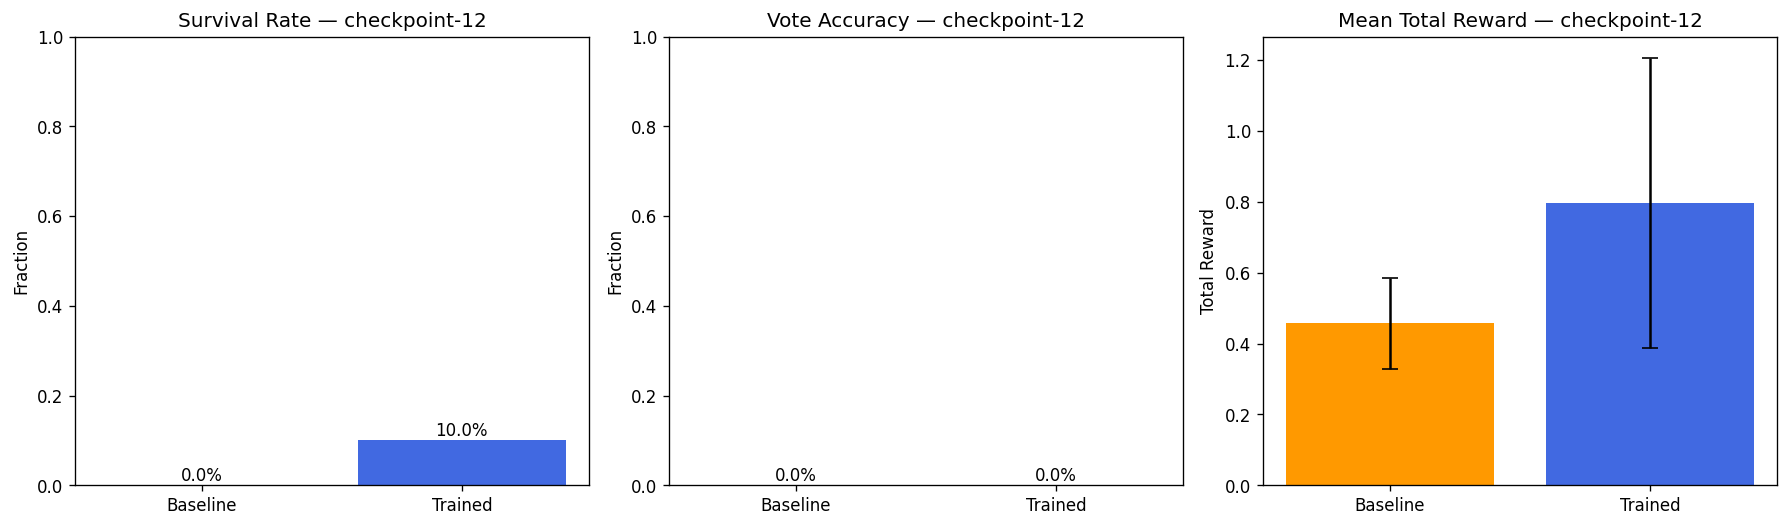
\includegraphics[width=0.92\textwidth]{figures/eval_step_0012_bars.png}
  \caption{Step-12 eval. Baseline ($n_b{=}30$) vs.\ trained ($n_t{=}10$) on the three
           primary metrics: survival rate, vote accuracy, and mean total episode
           reward (with $\pm 1\sigma$ on the reward panel). Source:
           \texttt{noanya/zombiee/eval\_results/eval\_step\_0012\_bars.png},
           generated by \texttt{notebooks/eval\_colab.ipynb} cell~10.}
  \label{fig:bars}
\end{figure}

\begin{figure}[h]
  \centering
  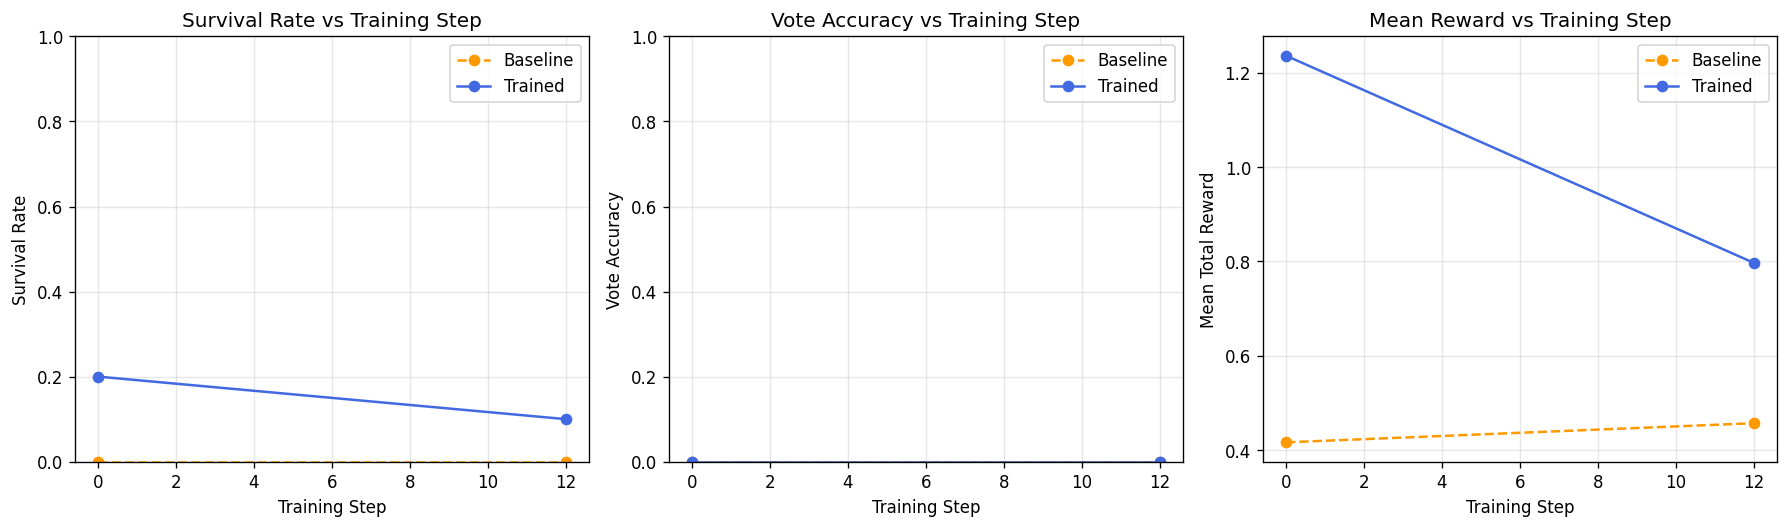
\includegraphics[width=0.92\textwidth]{figures/eval_history.png}
  \caption{Cross-checkpoint trend across the two completed evaluations: the
           partial-snapshot eval at $\approx$step~10 (Hub root, 2026-04-25T05:38\,UTC,
           $n_t{=}5,\ n_b{=}20$) and the proper step-12 eval
           (2026-04-25T08:14\,UTC, $n_t{=}10,\ n_b{=}30$). Step-12 is the
           headline; step-10 was a within-window sanity check, not a separate
           run. Both evaluations show positive deltas vs.\ baseline; step-12
           lands at a more conservative point estimate (survival 10\% vs.\ 20\%,
           reward $0.80$ vs.\ $1.24$) but with a larger sample.}
  \label{fig:history}
\end{figure}

\subsection{Behavioural Analysis}

\paragraph{Full-episode survival.}
In one of the ten trained-policy episodes (eval ep~2), the policy completed the
entire 100-step horizon with at least one healthy agent alive at termination,
accumulating a total reward of \textbf{1.965}. The remaining nine episodes
terminated mid-game with shorter survival but consistently above-baseline
rewards (mean $0.667$ on the non-survivor subset vs.\ $0.457$ for the
$n_b{=}30$ random baseline). The bimodal outcome distribution --- one full
survival, nine mid-episode deaths --- suggests the policy has acquired a
\emph{partial} strategy that closes the loop when initial conditions are
favourable but is brittle to early adverse zombie spawns or hunger
trajectories. With $n_t{=}10$ this is still small-$N$, but the existence of
a 100-step episode is evidence the policy can in principle solve the task.

\paragraph{Emergent theory-of-mind broadcast.}
Representative trained-agent broadcast:
\begin{quote}\itshape
  ``I notice A2 is very hungry and may be infected soon.''
\end{quote}
Emitted at $t{<}30$ in an episode where A2 was the infected agent. Concrete
reasoning chain: identified a specific peer (A2), referenced the correct
behavioural cue (hunger rate), made the right inference (infected), and
broadcast under the 40-char cap (truncated from 51 chars in the eval pipeline,
preserving diagnostic content). Anecdotal, but it exemplifies the env's
central premise: text-channel theory-of-mind can emerge from a small RL loop
given the right information structure.

% ============================================================================
%  6. DISCUSSION
% ============================================================================
\section{Discussion}
\label{sec:discussion}

\subsection{What Worked}
\begin{itemize}[leftmargin=*]
  \item \textbf{OpenEnv compliance was first-pass.} All four R1 validator traps
        (reward bounds, health endpoint string, per-step reward, determinism)
        were preempted via the patterns codified in
        \texttt{.planning2/01\_OPENENV\_PATTERNS.md}.
  \item \textbf{Format learning is complete.} 100\% JSON parse rate across the
        trained eval. Zero unparseable outputs.
  \item \textbf{Reward direction is unambiguous.} Mean total reward
        ($0.80$ vs.\ $0.46$, $1.7\!\times$) and mean episode length
        ($37.6$ vs.\ $19.1$ steps, $2.0\!\times$) both improved well beyond the
        small-sample noise floor. The trained policy keeps agents alive, on
        average, roughly twice as long as random --- evidence the policy is
        discovering survival strategy, not just action grammar.
  \item \textbf{Cross-machine training resilience.}
        \texttt{hub\_strategy="every\_save"} with step-1 save cadence made
        Colab/Kaggle disconnects cost $<$\,20\,min of compute; any of three
        runners (Colab, Kaggle, DGX) could resume from the same Hub repo
        (\texttt{noanya/zombiee}).
\end{itemize}

\subsection{Limitations}
\label{sec:limitations}
\begin{itemize}[leftmargin=*]
  \item \textbf{Reward-signal weakness.} The reward hook scores only the
        \emph{first} model action; the remaining $\sim$99 steps are uniform
        random. GRPO group reward variance ($\sigma{=}0.014$) is therefore
        dominated by rollout RNG, weakening the policy gradient --- consistent
        with the small KL drift and tiny grad norms observed in training.
  \item \textbf{Behavioural-cue leakage.} \texttt{infection.py} emits explicit
        text cues (\textit{``A1 is unusually hungry''}) into observations. A
        trained agent can string-match these rather than reason about hunger
        trajectories. A natural follow-up is to replace literal cues with
        noisy, false-positive-prone hints (see Future Work).
  \item \textbf{Sample size.} $n_t{=}10$ gives a 95\% binomial CI for the
        survival rate of $\approx[0.25\%,\ 44.5\%]$ around $1/10$. The reward
        and episode-length deltas are large relative to within-class
        $\sigma$, so those comparisons are more robust than the survival
        headline. Larger $N$ (e.g.\ $50$) was infeasible in the 24-hour
        hackathon budget at $\sim$3\,min per LLM-driven episode.
  \item \textbf{Single map.} All evaluation episodes use the same fixed grid;
        generalisation to varied layouts is untested.
\end{itemize}

% ============================================================================
%  7. FUTURE WORK
% ============================================================================
\section{Future Work}
\label{sec:future}

The architecture is deliberately additive-friendly: the OpenEnv contract,
post-mortem mechanism, and LoRA pipeline all generalise to a richer follow-up
with no breaking changes to the action space or reward interface. Concrete
directions we plan to explore:

\begin{itemize}[leftmargin=*,nosep]
  \item \textbf{Larger team, multiple hidden roles.} Five agents with two
        starting infected (e.g.\ a biter that spreads infection on contact
        and a saboteur that depletes shared resources) increases the
        social-deduction signal-to-noise ratio.
  \item \textbf{Iterated voting.} Vote phases at $t\in\{30,60,90\}$ instead
        of a single $t{=}50$ vote let the policy correct an early wrong vote.
  \item \textbf{Resource scarcity \& inventory.} Distinct food / water /
        medicine resources with a 3-slot inventory force inter-agent
        coordination beyond pure broadcast.
  \item \textbf{Day/night and zombie waves.} A visibility cycle plus
        scheduled wave spawns at $t\in\{25,50,75\}$ stretches the
        long-horizon survival signal further.
  \item \textbf{Noisy behavioural cues.} Replace the literal-string cue
        leakage flagged in §\ref{sec:limitations} with false-positive-prone
        hints, forcing the policy to reason over trajectories rather than
        match strings.
  \item \textbf{Zero-shot transfer experiment.} Because the upgrades are
        action-space-additive, the v1 LoRA can be evaluated unmodified on
        the richer environment. The proposed comparison is
        \emph{v1-LoRA-zero-shot} vs.\ \emph{from-scratch} vs.\
        \emph{warm-started}; the latter two require additional GRPO time.
\end{itemize}

% ============================================================================
%  8. CONCLUSION
% ============================================================================
\section{Conclusion}

SurviveCity demonstrates a working instance of cross-episode failure-replay
learning in a multi-agent LLM setting, with strict OpenEnv compliance. The
post-mortem mechanism is a principled alternative to LLM-as-judge or full
episodic memory and respects the OpenEnv validator's deterministic-reward
constraint. After 12 GRPO steps ($\approx$3\,h\,53\,min on a Colab T4), the
step-12 evaluation gives \textbf{100\% action-grammar compliance},
\textbf{$1.7\!\times$ baseline mean reward} ($0.80$ vs.\ $0.46$),
\textbf{$2.0\!\times$ baseline episode length} ($37.6$ vs.\ $19.1$ steps),
and survival rate $0\%\rightarrow 10\%$, with one $n_t{=}10$ episode reaching
full 100-step survival (reward $1.97$). The largest remaining bottleneck is
the simplified reward hook (one model action then random rollout); the
follow-up directions in §\ref{sec:future} address this with multi-step model
rollouts and an action-space-additive richer environment that lets the v1
LoRA be evaluated zero-shot for transfer measurement.

% ============================================================================
%  LINKS
% ============================================================================
\section*{Project Artefacts}

\begin{itemize}[leftmargin=*,nosep]
  \item Source code: \url{https://github.com/SirjanSingh/zombiee}
  \item Hugging Face model + checkpoints + eval results:
        \url{https://huggingface.co/noanya/zombiee}
  \item Hugging Face Space (live env): \textit{(deployment pending)}
  \item 2-min demo video: \textit{(recording pending)}
  \item Training run TensorBoard log: \url{https://huggingface.co/noanya/zombiee/tree/main/runs/Apr25_02-16-25_c3b2d410c5bd}
  \item Step-12 eval results: \url{https://huggingface.co/noanya/zombiee/blob/main/eval_results/eval_step_0012.json}
  \item Cross-checkpoint eval history: \url{https://huggingface.co/noanya/zombiee/blob/main/eval_results/eval_history.png}
  \item Colab training notebook: \texttt{notebooks/train\_colab.ipynb}
  \item Colab eval notebook:     \texttt{notebooks/eval\_colab.ipynb}
\end{itemize}

% ============================================================================
%  BIBLIOGRAPHY
% ============================================================================
\bibliographystyle{plain}
\bibliography{refs}

\end{document}
